\documentclass[11pt,a4paper]{article}
\usepackage{amsmath,amssymb,graphicx,booktabs,geometry}
\usepackage{float}
\geometry{margin=1in}

\title{Modeling Locust Swarming with a Continuous-Activity ODE Model}
\author{Bar Jacobi \& Amy Vogel}
\date{\today}

\begin{document}
\maketitle

\section{Introduction}

Locusts are well-known for their collective motion, where individuals alternate between solitary and gregarious phases. Modeling this behavior has been an active area of research, ranging from simple self-propelled particle (SPP) models to biologically detailed pause-and-go dynamics \cite{ariel2015locust}.  

In this project, we implement a minimal ODE-based model of locust collective motion. Each agent is represented by its position, heading, and an internal \emph{continuous activity variable}. This variable replaces the discrete pause/go states used in previous models. Biologically, it can be interpreted as a measure of locomotor readiness: $a=0$ corresponds to being fully paused, $a=1$ to full walking, and intermediate values to gradual activation or partial movement. Such a representation is consistent with observations that locusts accelerate gradually and that their responsiveness to neighbors increases smoothly with group density.  

Our goals are to (i) situate the model in relation to existing work, (ii) clarify its assumptions and simplifications, (iii) define all parameters and variables with units, and (iv) evaluate robustness via parameter sweeps and heatmaps.

\section{Relation to Existing Models}

Ariel and Ayali (2015) review several frameworks for modeling locust collective motion:
\begin{itemize}
    \item The \textbf{Czirók model}, a 1D variant of the Vicsek self-propelled particle model, where individuals align to neighbors within a radius plus noise.
    \item The \textbf{Buhl model}, a refinement that adds persistence in direction, fitted to ring-arena experiments.
    \item The \textbf{Pause-and-go model}, where locusts switch between discrete moving and paused states, based on experimental observations of intermittent locomotion.
    \item \textbf{Escape-and-pursuit models}, motivated by cannibalism hypotheses, where individuals pursue those ahead and flee from those behind.
\end{itemize}

Our approach is closest to the Vicsek/Czirók family of models but introduces an important modification. Instead of discrete pause/go states, we use a continuous-valued activity variable $a \in [0,1]$. This captures the same social dependence as the pause-and-go model but softens it into a smooth dynamical variable. The advantage is twofold: (i) it allows a natural biological interpretation as varying degrees of locomotor activation, and (ii) it yields a mathematically tractable ODE formulation suitable for robustness analysis.

\section{Model Definition}

Each locust is described by:
\begin{itemize}
    \item \textbf{Position:} $(x,y)$, coordinates in a periodic square domain of side length $L$ (m).
    \item \textbf{Direction:} $\theta$, orientation of movement (radians).
    \item \textbf{Activity:} $a \in [0,1]$, continuous locomotion variable (0 = paused, 1 = fully moving).
\end{itemize}

\subsection{Activity dynamics}
Activity relaxes toward a sigmoid function of neighbor count $n_i$:
\[
\frac{da_i}{dt} = -\frac{1}{\tau_a}\Big(a_i - \sigma(\beta_0 + \beta_1 n_i)\Big),
\]
where $\tau_a$ (s) is the relaxation timescale, $\beta_0$ is the baseline bias, and $\beta_1$ is the social activation gain.

The sigmoid represents biologically plausible graded transitions: in many animal systems, movement does not engage instantly but ramps up. Speed, gait, and responsiveness transition continuously. For instance, studies of human gait show that increases in walking speed yield smooth changes in joint kinematics and ground-reaction forces, rather than abrupt jumps \cite{fukuchi2019gait}. Our model's continuous activity variable is inspired by such gradual biomechanical activation, and offers a realistic, smooth analogue to the binary pause–go concept.


\subsection{Velocity}
Speed varies between minimum and maximum values depending on activity:
\[
v_i = v_{\min} + (v_{\max} - v_{\min}) a_i.
\]

\subsection{Direction dynamics}
Directions evolve by alignment with neighbors plus noise:
\[
\frac{d\theta_i}{dt} = \kappa \cdot \langle \sin(\theta_j - \theta_i)\rangle + \sqrt{2\eta}\,\xi,
\]
where $\kappa$ is alignment strength, $\eta$ is noise intensity (rad$^2$/s), and $\xi$ is Gaussian white noise.

\subsection{Domain}
Motion occurs in a square domain with periodic boundary conditions.

\section{Parameters and Variables}

\subsection{Mathematical parameters}

\begin{tabular}{@{}llll@{}}
\toprule
Symbol & Meaning & Units & Default \\
\midrule
$N$ & Number of locusts & count & 120 \\
$L$ & Domain size & m & 10 \\
$v_{\min}$ & Minimum speed & m/s & 0.01 \\
$v_{\max}$ & Maximum speed & m/s & 0.15 \\
$\kappa$ & Alignment strength & 1/s & 2.0 \\
$R$ & Vision radius & m & 1.0 \\
$\eta$ & Noise intensity & rad$^2$/s & 0.4 \\
$\beta_0$ & Baseline activity bias & --- & -1.0 \\
$\beta_1$ & Social activation gain & --- & 0.25 \\
$\tau_a$ & Activity relaxation time & s & 0.5 \\
\bottomrule
\end{tabular}

\subsection{Computational parameters}

\begin{tabular}{@{}llll@{}}
\toprule
Symbol & Meaning & Units & Default \\
\midrule
$dt$ & Simulation time step & s & 0.05 \\
$T$ & Total simulation time & s & 100 \\
seed & Random seed & --- & 42 \\
\bottomrule
\end{tabular}

\section{Robustness Analysis}

To test robustness, we ran parameter scans. For each case we measured the \textbf{polarization}:
\[
P = \sqrt{\Big(\frac{1}{N}\sum_i \cos \theta_i\Big)^2 + \Big(\frac{1}{N}\sum_i \sin \theta_i\Big)^2}.
\]

$P=0$ means complete disorder; $P=1$ means perfect alignment.

\subsection{Scan 1: $\kappa$ vs $R$}
Polarization rises sharply when both alignment strength and vision radius are above threshold values, similar to the phase transition seen in Vicsek models.

\begin{figure}[H]
    \centering
    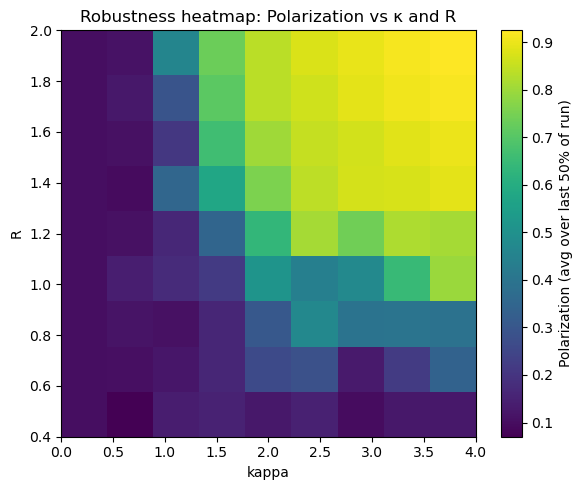
\includegraphics[width=0.5\textwidth]{k_vs_r.png}
    \caption{Polarization results for Scan 1 ($\kappa$ vs $R$). Stronger alignment and vision radius increase group order.}
    \label{fig:scan1}
\end{figure}

\subsection{Scan 2: $\kappa$ vs $\beta_1$}
With higher social activation $\beta_1$, swarms form more easily: polarization grows at lower $\kappa$ values. This shows that even a simple activity variable strongly shapes group order.

\begin{figure}[H]
    \centering
    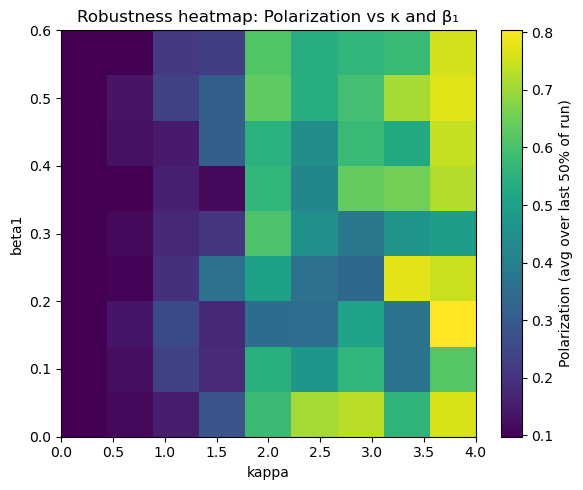
\includegraphics[width=0.5\textwidth]{k_vs_b1.png}
    \caption{Polarization across $\kappa$ vs $\beta_1$. Stronger social activation lowers the threshold for collective order.}
    \label{fig:scan2}
\end{figure}

\section{Discussion}

Our model differs from prior work in that it uses a continuous activity variable rather than a binary pause/go state. Biologically, this can be interpreted as a measure of \emph{locomotor readiness} or gradual acceleration: locusts do not always switch instantly between full pausing and full walking, but may exhibit intermediate levels of movement or responsiveness to neighbors. From a modeling perspective, this continuous formulation smooths out discontinuities, simplifies numerical analysis, and retains the threshold/saturation effects central to pause–and–go dynamics.  

Robustness analysis confirms that swarming arises only when alignment strength and social activation are sufficiently large, consistent with prior studies. While our model does not capture all biological details (e.g., discrete pausing, escape-and-pursuit asymmetries), it highlights the minimal ingredients necessary for collective order. According to Ariel and Ayali (2015), such simplified models are valuable for understanding general principles of swarm dynamics, even if they abstract away some biological realism.

\section{Conclusion}

We implemented and analyzed a continuous-activity ODE model of locust swarming. Our work shows that simple local rules (alignment, social activation, and noise) are sufficient to generate robust collective motion. By situating this model within the broader literature, we demonstrate both how it simplifies existing frameworks and what insights it contributes. The approach also emphasizes the importance of robustness checks and parameter documentation, ensuring reproducibility and interpretability.

\begin{thebibliography}{9}
\bibitem{ariel2015locust}
Ariel, G., \& Ayali, A. (2015). Locust collective motion and its modeling. \emph{PLoS Computational Biology}, 11(12), e1004522.
\bibitem{fukuchi2019gait}
Fukuchi CA, Fukuchi RK, Duarte M. (2019). Effects of walking speed on gait biomechanics in healthy participants: a systematic review and meta-analysis. \emph{Systematic Reviews}, 8, 153.
\end{thebibliography}

\end{document}
